\chapter{Interpolazione}
\section{B\'ezier}

Siano $P_i(x_i, y_i), i = 0, 1, n$, punti di controllo, la curva parametrica si forma:
\begin{align}
  Q_n(t) = \sum_{i=0}^n P_i f_i(t), \quad t \in [0, 1]
\end{align}

$f_i(t)$ sono opportune funzioni polinomiali scelte in modo tale che la curva abbia le seguenti proprietà:

\begin{itemize}
  \item $Q_n(0) = P_0$
  \item $Q_n(1) = P_n$
  \item La tangente in $P_0$ \`e parallela a $P_1 - P_0$
  \item La tangente in $P_n$ \`e parallela a $P_n - P_{n-1}$
\end{itemize}


Queste condizioni sono soddisfate assumendo come funzioni $f_i(t)$ i polinomi di Bernstein:

\begin{align}
  B_i^n(t) = \binom{n}{i} t^i (1-t)^{n-i}, \quad i = 0, 1, n
\end{align}

Dove la binomiale si calcola come:
\begin{align}
  \binom{n}{i} = \frac{n!}{i!(n-i)!}
\end{align}


Quindi la curva di B\'ezier \`e data da:
\begin{align}
  Q_n(t) = \sum_{i=0}^n P_i B_i^n(t), \quad t \in [0, 1]
\end{align}

\begin{figure}[h!]
  \centering
  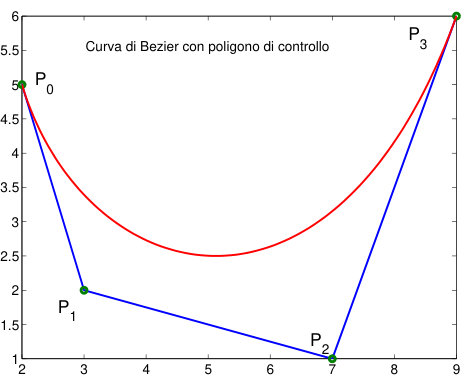
\includegraphics[width=0.4\linewidth]{images/curva_bazier_esempio.png}
\end{figure}



Spesso \`e necessario utilizzare pi\`u curve e per fare ci\`o si utilizzano i gradi di continuith\`a.

\begin{itemize}
  \item $C^0$, le due curve hanno un punto in comune (primo nodo della seconda curva coincide con l'ultimo della prima)
  \item $C^1$, le due curve hanno un punto in comune e la derivata prima \`e uguale in direzione e modulo
\end{itemize}

\subsection{Curve di B\'ezier razionali}

In questo caso si introduce un valore di peso per ogni punto di controllo, quindi la curva \`e data da:
\begin{align}
  Q_n(t) = \frac{\sum_{i=0}^n P_i w_i B_i^n(t)}{\sum_{i=0}^n w_i B_i^n(t)}, \quad t \in [0, 1]
\end{align}


\begin{figure}[h!]
  \centering
  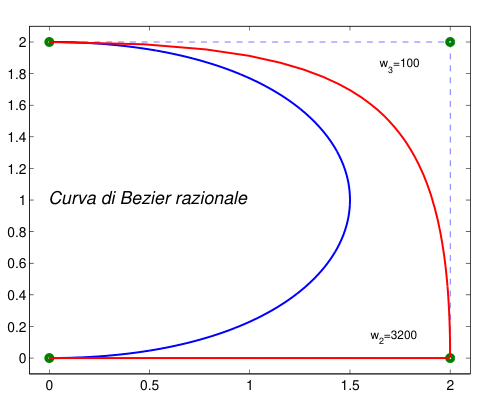
\includegraphics[width=0.4\linewidth]{images/bazier_pesato_esempio.png}
\end{figure}



\section{Interpolazione di funzioni in pi\`u variabili}
Sapendo che il polinomio Lagrangiano \`e:
\begin{align}
  L_{ij}(x, y) = L_i(x) L_j(y)
\end{align}

Il polinomio interpolante \`e:
\begin{align}
  p_{n, m}(x, y) &= \sum_{i=0}^n \sum_{j=0}^m f(x_i, y_j) L_{ij}(x, y) \\
  &= \sum_{i=0}^n \sum_{j=0}^m f(x_i, y_j) L_i(x) L_j(y)
\end{align}
